\documentclass[1p,sort&compress]{elsarticle}
\usepackage{amsmath,amssymb}
\usepackage{breqn}
\usepackage{bbold}
\usepackage{booktabs}
\usepackage{graphicx}
\usepackage[utf8]{inputenc}
\usepackage[T1]{fontenc}
\usepackage{caption}
\usepackage{siunitx}
\usepackage{hyperref}
\usepackage[labelfont=bf,textfont={sl,bf},lofdepth,lotdepth]{subfig}
\usepackage{xspace}
\usepackage{color}
\usepackage{proba}
\usepackage[usenames,dvipsnames,svgnames,table]{xcolor}
\usepackage{cleveref}
\usepackage{paralist}
\usepackage[title,titletoc,toc]{appendix}
%%%%%%%%%%%%%%%%%%%%%%%%%%%%%%%%%%%%%%%%%%%%%%%%%%%%%%%%%%%%%%%%%%%%%%%%%%%%%%%%%%%%%%%%%%
%                                  MODIFICACIONES                                        %
%%%%%%%%%%%%%%%%%%%%%%%%%%%%%%%%%%%%%%%%%%%%%%%%%%%%%%%%%%%%%%%%%%%%%%%%%%%%%%%%%%%%%%%%%%
\oddsidemargin=1cm
\textwidth=14cm
%%%%%%%%%%%%%%%%%%%%%%%%%%%%%%%%%%%%%%%%%%%%%%%%%%%%%%%%%%%%%%%%%%%%%%%%%%%%%%%%%%%%%%%%%%
%                                 FORMATOS                                               %
%%%%%%%%%%%%%%%%%%%%%%%%%%%%%%%%%%%%%%%%%%%%%%%%%%%%%%%%%%%%%%%%%%%%%%%%%%%%%%%%%%%%%%%%%%
\DeclareMathAlphabet{\mathpzc}{OT1}{pzc}{m}{it}
\newtheorem{dfn}{Definition}
\newtheorem{thm}{Theorem}[section]
\newtheorem{pro}{Proposition}[section]
\newtheorem{lem}{Lemma}[section]
\newtheorem{definition}{Definition}[section]
\newtheorem{corollary}{Corollary}[section]
\newtheorem{consequence}{CONSEQUENCE}[section]
\newtheorem{remark}{Remark}[section]
\newtheorem{example}{\bf Example}[section]
\newtheorem{proof}{\bf Proof}[section]
\newtheorem{assumption}{Assumption}[section]
\newproof{pf}{Proof}
\newproof{Proof}{Proof}
\providecommand*{\lemautorefname}{Lemma}
\providecommand*{\thmautorefname}{Theorem}
\providecommand*{\assumptionautorefname}{Assumption}

\newcommand{\fin}{\vrule height3pt width3pt depth2pt}
\newcommand{\normL}[1]{\left[\mathbb{E}\left|#1\right|^2\right]^{1/2}}
\newcommand{\ms}[1]{\mathbb{E}\left|#1\right|^2}
\newcommand{\mep}[1]{\mathbb{E}|#1|^p}
\newcommand{\m}[1]{\mathbb{E}#1}
\newcommand{\Prob}[1]{\mathbb{P}\left[#1\right]}
\newcommand{\meanp}[2]{\mathbb{E}\left|#1\right|^{#2}}
\newcommand{\condexp}[2]{\mathbb{E}\left[#1|#2\right]}
\newcommand{\lftrght}[3]{\left#2 #1\right #3}\DeclareMathOperator{\tr}{tr}
\newcommand{\innerprod}[2]{\left\langle#1, #2\right\rangle}
\newcommand*{\eg}{e.g.,\xspace}
\newcommand*{\ie}{i.e.,\xspace}
\newcommand*{\todo}[1]{\textcolor{BrickRed}{#1}\\}
\newcommand{\crefrangeconjunction}{--}
\crefrangeformat{equation}{(#3#1#4)--(#5#2#6)}
\DeclareMathOperator{\diag}{diag}
\DeclareMathOperator*{\as}{a.s.}
%opening
\begin{document}
	\begin{frontmatter}
		\title{
			Strong Convergence and Almost Sure Stability of an Explicit Steklov Method
			for SDE under non-globally Lipschitz Coefficients.
		\tnoteref{t1}
		}%,t2}}
		\tnotetext[t1]{
			This work has been partially
			supported by CONACYT project *****
		}
		\author[sj]{S. D\'{\i}az-Infante}
		\ead{sauld@cimat.mx}
		\author[sj]{S. Jerez}
		\ead{jerez@cimat.mx}
		\address[sj]{Split Step Linear Steklov Method 
		Department of Applied Mathematics, CIMAT, Guanajuato, Gto., Mexico,
		36240.
		}
		\begin{abstract}
			We present an explicit and easily implementable numerical method for
			solving stochastic differential equations (SDEs) with non-globally Lipschitz
			coefficients. The underlying method converges strongly with standard 
			one-half order. A linear version of the Steklov average supports our new solver. Also, we study
			the almost sure asymptotic stability, and in  order to emphasize the 
			performance of the Steklov discretization we use models from population dynamics 
			and finance.
		\end{abstract}
		\begin{keyword}
			stochastic differential equations;
			explicit methods; convergence; asymptotic stability;
			BD simulation; logistic equation.
		\end{keyword}
	\end{frontmatter}
	\section{Introduction}
		%	Applications of Monte Carlo type simulations \cite{Glasserman2004,Giles2008} as  Brownian Dynamics \cite{Cruz2012}
%require  fast numerical methods with low computational cost --- excluding the use of 
%implicit schemes in the majority of cases.
%The EM method is the most popular in such  
%simulations due to its simple algebraic structure, cheap computational cost and acceptable convergence rate 
%under global Lipschitz conditions. 
%However, if the drift or diffusion coefficient of stochastic 
%differential equation  is super-linear, then the EM approximation 
%diverges  in the mean square sense \cite{Hutzenthaler2009, Hutzenthaler2012b}. 
%In most applications, the coefficients of the stochastic  models in finances, biology or physics 
%have locally Lipschitz coefficients with super-linear growth. 
%Therefore, recent research has been focused on modifying the EM method to obtain strong convergence  under these 
%conditions keeping its simple structure and  its low computational cost. In the last years, 
%several methods have been developed in this direction:  the family of  Tamed schemes
%\cite{Hutzenthaler2012a, Wang2011, Zong2014,Hutzenthaler2015,Sabanis2015}, 
%a special type of balanced method \cite{Tretyakov2013},  the stopped scheme \cite{Liu2013a} and 
%a truncated Euler method  \cite{Mao2015}.
%In these works, the strong convergence of the proposed method
%is proved using the theory developed by Higham, Stuart and 
%Mao in \cite{Higham2002b} or by means of  the new approach given by  Hutzenthaler and Jentzen in 
%\cite{Hutzenthaler2015}.
%Both techniques obtain the property of  strong convergence by proving boundedness moments of the numerical and 
%analytical solution of the underlying SDE. In spite of the recent work in this subject,  it is still necessary
%to get more accurate numerical methods for SDE under super-linear growth and 
%non-globally Lipschitz coefficients.

	In this chapter, we develop an explicit method based on a linear version  of the Steklov method proposed 
in  \Cref{ch:Chapter3}. We consider the vector It\^o stochastic differential equation
\begin{equation}\label{eqn:SDE1}
	dy(t)
	 =f(y(t))dt + g(y(t))dW(t), \quad 0\leq t\leq T,
	\quad y(0)=y_0,
\end{equation}
where $(f^{(1)},\dots, f^{(d)}):\R^d \to \R^d$ is one sided Lipschitz and 
$g = (g^{(j,i)})_{j\in \{1,\dots,d\}, i\in\{1,\dots, m\}}:\R^d \to \R^{d\times m}$ is global Lipschitz. 
Also we assume 
that  each component function $f^{(j)}$  can be written of the form
\begin{equation}\label{eqn:AlternativeConstruction}
	f^{(j)}(x) = a_j(x) x^{(j)} + b_j (x^{(-j)}), 
\end{equation}
where $a_j$ and	$b_{j}$ are two scalar 	functions in  $\R^d$ 
and $x^{(-j)} = \left( x^{(1)},\dots,x^{(j-1)},x^{(j+1)},\dots x^{(d)}\right)$.%
	\section{Existence and uniqueness of the solution}
		%
\begin{thm}[{
		%\citeauthor{Mao2013}
	 \cite[Thm. 2.2]{Mao2013}}]
	Let \Cref{ass:OSLC} holds. Then for all $y(0)=y_0\in \mathbb{R}^d$ given, there exist a 
	unique global solution $\{y(t)\}_{t\geq 0}$ to SDE\eqref{eqn:SDE1}. Moreover, the solution has the 
	following properties for any $T>0$,
	\begin{equation*}
		\ms{y(T)}< 
		\left(
			|y_0|^2 +2\alpha T 
		\right)\exp(2\beta T),
	\end{equation*}
	and
	\begin{equation*}
	\Prob{\tau_n\leq T}
	\leq \frac{
		\left(
		|y_0|^2 +2\alpha T 
		\right)
		\exp(2\beta T)
	}{n},
	\end{equation*}
	where $n$ is any positive integer and 
	%\begin{equation*}
	$\tau_n := \inf \{ t\geq 0 : |y(t)|>n\}$.
	%\end{equation*}
\end{thm}
%
\begin{thm}[
		%\citeauthor{Mao2007} 
		{\cite[Thm. 2.4.1]{Mao2007}}
	]
	\label{thm:MaoCoercive}
	Let $p\geq 2$ and $x_0\in L^p(\Omega, \mathbb{R}^d)$. Assume that there exits a constant $C>0$
	such that for all $(x,t)\in \mathbb{R}^d\times [t_0,T]$,
	\begin{equation*}
	\innerprod{x}{f(x,t)}+\frac{p-1}{2}|g(x,t)|^2 \leq C(1+|x|^2).
	\end{equation*}
	Then
	\begin{equation*}
	\m|y(t)|^p
	\leq
	2^{\frac{p-2}{2}}
	\left(
	1 + \m|y_0|^p
	\right)\exp({Cpt}) \quad \text{ for all } t\in[0,T].
	\end{equation*}
\end{thm}
%
\begin{lem}[
	{
		%\citeauthor{Higham2002b}
		\cite[Lem 3.2]{Higham2002b}}
	]
	\label{lem:MomentBound}
	Under \Cref{ass:OSLC}, for each $p\geq 2$, there is a $C=C(p,T)$ such that
	\begin{equation*}
	\EX{\sup_{0\leq t \leq T}|y(t)|^p}\leq C \left(1+\mep{y_0}\right).
	\end{equation*}
\end{lem}
%
	\section{Construction of the SSSM}
		%
	For simplicity, we begin the construction of the Linear Steklov method (\SM) considering the scalar case of SDE 
\eqref{eqn:SDE1}, that is, when $d=m=1$, also, to shorten notation we use $a,b$ instead $a_j,b_j$. 
Tough this ideas, we will generalize to higher dimensions.
Let $0=t_0 < t_1< \cdots < t_N=T$ a partition of the interval $[0,T]$ with constant step-size $h=T/N$ and such that
$t_k=kh$ for $k=0,\ldots, N$. The main idea of the  \SM approximation  consists in 
estimating the drift coefficient of \eqref{eqn:SDE1}  by
\begin{equation}
	f(y(t)) \approx 
		\varphi_{f}(y(t_{\eta_{+}(t)})) =
		\left(
			\frac{1}{y(t_{\eta_+(t)})-y(t_{\eta (t)})}
			\bigint \limits
_				{y(t_{\eta(t)})}^{y(t_{\eta_+(t)})}
					\frac{du}
						{
							a(y(t_{\eta(t)}))u
							+b
						}
	\right)^{-1}, \qquad t\in [0,T],
\end{equation}
where
\begin{align*}
	\eta(t) &:=
	k\text{  for } t\in [t_k, t_{k+1}), \quad k\geq 0,\\
	\eta_{+}(t) &:= 
	k+1  \text{ for } t\in [t_k, t_{k+1}), \quad k\geq 0.
\end{align*}
So we define the \SM method for the scalar version of the SDE \eqref{eqn:SDE1} using a split-step formulation as follows
\begin{align}
	Y_k^{\star} &= Y_k + h \varphi_f(Y^{\star}_k), \label{eqn:SSLSM1}\\
	Y_{k+1}	&= Y_k^{\star} + g(Y_k^{\star})\Delta W_k \label{eqn:SSLSM2},
\end{align}
with $Y_0=y_0$ and  $\varphi_{f}\left(Y_k^{\star}\right)$ defined by 
\begin{equation}
	\varphi_{f}\left(Y_k^{\star}\right)
	=
		\left(
			\frac{1}{Y_{k}^{\star}-Y_{k}}
			\int 
			%\limits
			_{Y_{k}}^{Y_{k}^{\star}}
				\frac{du}
				{
					a(Y_k)u
					+b
				}
	\right)^{-1}
\end{equation}
This scheme combines a split-step technique with a linear version of an exact deterministic 
method see \cite{Diaz-Infante2015,Matus2005}. 
In detail, first we compute the discrete value $Y^{\star}_k$ using the Linear Steklov approximation \eqref{eqn:SSLSM1},
and next, $Y_{k+1}$ is obtained by adding the stochastic increment $g(Y_k^\star)\Delta W_k$.

	To higher dimensions, we adapt the same split step scheme \crefrange{eqn:SSLSM1}{eqn:SSLSM2} as follows. 
For each component equation $j\in\{1, \ldots,  d\}$, on the iteration $k\in\{1, \ldots,  N\}$ take
\begin{align}
	a_{j,k} &=
	a_j
	\left(
		Y^{(1)}_{k},
		\ldots, Y^{(d)}_{k}
	\right),
	&
	b_{j,k} =
	b_{j}
	\left(
			Y^{(-j)}_k
	\right).
\end{align}
So, define  
$
	\varphi_{f}(Y_k^{\star})=
		\left(
			\varphi_{f^{(1)}}(Y_k^{\star}),
			\ldots,
			\varphi_{f^{(d)}}(Y_k^{\star})
		\right)
$
by
\begin{equation}
	\varphi_{f^{(j)}}\left(Y_k^{\star}\right)
		=
		\left(
			\frac{1}{Y_{k}^{\star(j)}-Y_{k}^{(j)}}
			\int 
			%\limits
				_{Y_{k}^{(j)}}^{Y_{k}^{\star(j)}}
				\frac{du}
				{
					a_{j,k} u
					+b_{j,k}
				}
		\right)^{-1}.
\end{equation}
%
	It is worth mentioning that even this formulation is semi implicit, we always can derive a explicit version. 
The next result deals with this issue. To simplify notation, we define  $A^{(1)}= A^{(1)}(h,u)$,  $A^{(2)}=A^{(2)}(h,u)$  and $b=b(u)$ by 
\begin{align}\label{eqn:SolutionFunctions}	
	A^{(1)}&:=
		\begin{pmatrix}
			e^{ha_1(u)} & \multicolumn{2}{c}{\text{\kern0.5em\smash{\raisebox{-1ex}{\huge 0}}}} \\
			&\ddots\\
			\multicolumn{2}{c}{\text{\kern-0.5em\smash{\raisebox{0.95ex}{\huge 0}}}} 
			& e^{ha_d(u)}
		\end{pmatrix},
		\notag
		\\
		%	
	A^{(2)}&:=
	\begin{pmatrix}
		\left(
			\displaystyle
			\frac{e^{ha_1(u)} - 1}{a_1(u)}
		\right)\1{E_1^c}	& 
		\multicolumn{2}{c}{\text{\kern0.5em\smash{\raisebox{-1ex}{\huge 0}}}}\\
		 & \ddots&\\
		\multicolumn{2}{c}{\text{\kern0.5em\smash{\raisebox{-1ex}{\huge 0}}}}&
		\left(
			\displaystyle
			\frac{e^{ha_d(u)} - 1}{a_d(u)}
		\right)\1{E_d^c}% + h \1{E_i} 
	\end{pmatrix}
	+h
	\begin{pmatrix}
		\1{E_1} & \multicolumn{2}{c}{\text{\kern0.5em\smash{\raisebox{-1ex}{\huge 0}}}}\\
		&\ddots &\\
		\multicolumn{2}{c}{\text{\kern0.5em\smash{\raisebox{-1ex}{\huge 0}}}} &
		\1{E_d}
	\end{pmatrix},\\	
	E_j&:=\{x \in \R^d: a_j(x)=0\} , \qquad 
	b(u):= \left(
		b_1(u^{(-1)}), \dots , b_d(u^{(-d)})
	\right)^T.		
	\notag
\end{align}
	Also we will need the following results from \cite[Thm 2.1]{Lawlor2012}, \cite[Thm. 1]{FineAIandKass1966}.
The first theorem will help us  with the singularities of set $E_j$ in the case where all elements of this set
are limit points. 
\begin{thm}[Multivariate L'h\^{o}pital's Rule] \label{thm:Lawlor}
	Let $\mathcal{N}$ be a neighborhood in $\R^2$ containing a point $\mathbf{q}$ at which
	two differentiable functions $f:\mathcal{N}\to \R$ and $g:\mathcal{N}\to \R$ are zero.
	Set 
	$$
		C=\{x \in \mathcal{N}: f(x)=g(x)=0 \},
	$$
	and suppose that $C$ is a smooth curve through $\mathbf{q}$.
	
	Suppose	there exist a vector $\mathbf{v}$ not tangent to $C$ at $\mathbf{q}$
	such that the directional derivative $D_{\mathbf{v}}g$ of $g$ in the direction of $\mathbf{v}$ is never zero
	within $\mathcal{N}$. Also we assume that $\mathbf{q}$ is a limit point of $\mathcal{N}\setminus C$. Then
	\begin{equation*}
		\lim_{(x,y)\to \mathbf{q}}
		\frac{f(x,y)}{g(x,y)} =
		\lim_{
				\substack{
					(x,y)\to \mathbf{q}\\ 
					(x,y)\in \mathcal{N} \setminus C
				}
		}
		\frac{D_{\mathbf{v}} f }{D_{\mathbf{v}} g}
	\end{equation*}
	if the latter limit exist.
\end{thm}
For the second auxiliary we will need the following concepts.
\begin{dfn}[Directional derivative referred at a point]
	Let $u,\mathbf{q}\in \R^2$ and $\alpha$ the positive angle respect to the $x$-axis and the segment
	$\overline{u \mathbf{q}}$.	We denote by 
	\begin{align*}
		f_{\alpha}(u) &= 
			\cos(\alpha) 		
			\frac{\partial f}{\partial u^{(1)}}(u) + 
			\sin(\alpha)
			\frac{\partial f}{\partial u^{(2)}}(u) 
			= \frac{ \innerprod{q-u}{\nabla f(u)}}{|u-q|}			
	\end{align*}
	the \emph{directional derivative respect to the point $\mathbf{q}$ on $u$}.
\end{dfn}
\begin{dfn}[Star-like set]
	A set $S\subset \R^2$ is \emph{star-like} with respect a point $\mathbf{q}$, if for each point $s \in S$ the open 
	segment $\overline{s \mathbf{q}}$ is in $S$.
\end{dfn}
%
Whit this in mine, second theorem give us a way to analyze isolated singularities.
\begin{thm}\label{thm:Fine}
	Let $\mathbf{q}\in \R^2$ and let $f$,$g$ be functions whose domains include a set $S\subset \R^2$ which is 
	star-like 
	with  respect to the point $\mathbf{q}$. Suppose that on $S$ the functions are differentiable and that
	the directional derivative of $g$ with respect to $\mathbf{q}$ is never zero. With the understanding that all 
	limits are taken from within on $S$ at $\mathbf{q}$ and if
	\begin{enumerate}[(i)]
		\item 
			$f(\mathbf{q})=g(\mathbf{q})=0$,
		\item
			$
				\displaystyle
				\lim_{x \to \mathbf{q}}
				\frac{f_{\alpha}(x)}{g_{\alpha}(x)} = L,	
			$
	\end{enumerate}
	then
	$$
		\lim_{x \to \mathbf{q}}
		\frac{f(x)}{g(x)} = L.
	$$
\end{thm}
%
With this on mind, we additionally require the following. 
\begin{hypothesis}\label[hypothesis]{ass:ajBound} %\label{as:aiFunctions}
	For each component function $f^{(j)}:\R^d:\to \R$ %$j \in \{1, \dots, d \}$,
	with $j \in \{1,\dots, d\}$:
	\begin{enumerate}[({A}-1)]
		\item\label{ass:FunctionStructure}
		There are two locally Lipschitz functions of 
		class $C^1(\R^d)$ denoted by
		$a_j:\mathbb{R}^{d} \to \mathbb{R}$ and
		$b_{j}:\mathbb{R}^{d-1} \to \mathbb{R}$ such that 
		the $j$-component of the drift function can be rewritten 
		as in \eqref{eqn:AlternativeConstruction}.
		\item\label{a}
		There is a positive constant $L_a$ such that
		$$
		a_{j}(x) \leq L_a, \qquad\forall x\in \R^d.
		$$
		\item Each function $b_j(\cdot)$ satisfies the linear growth condition
		\begin{equation*}\label{eqn:bjLinearGrowthCondition}
		|b_j(x^{(-j)})|^2 \leq L_{b}(1+|x|^2) , \qquad \forall x\in \R^d.
		\end{equation*}
	\end{enumerate}
\end{hypothesis}

\begin{hypothesis} \label{ass:HypThmSingularities}
	The set $E_j:=\{x\in \R^{d}: a_j(x)=0\}$ satisfies either:
	\begin{enumerate}[(i)]
		\item
			All point $q \in E_j$ is a non isolated zero of $a_j$ and:
			\begin{itemize}
				\item the set 
					$$
						D:=\{u \in B_r(q): e^{ha_j(u)}-1=a_j(u)= 0\},
					$$ 
					is a smooth curve through $q$. 
				\item
					The canonical vector $e_j$ is not
					tangent to $D$.
				\item
					For each $q \in E_j$, there is an open ball with center
					on $q$ and radio $r$ $B_r(q)$, such that  
					and
					$$
						a_j\neq 0, \qquad
						\frac{\partial a_j(u)}{\partial u^{(j)}} \neq 0 ,\qquad 
						\forall u \in B_r(q)
						\setminus D.
					$$	
				%				
				%				\item
				%					The limit
				%					$$
				%						\lim_{
				%							\substack{
				%								u\to u^*\\ 
				%								u \in B_r(q) \setminus D
				%							}
				%						}
				%						\frac{e^{h a_j(h)} \frac{\partial a_j(u)}{\partial u^{(j)}}}{\frac{\partial a_j(u)}{\partial 
				%						u^{(j)}}}
				%					$$
				%					
			\end{itemize}	
		\item
			All point $q \in E_j$ is a isolated zero of $a_j$ and:
			\begin{itemize}
				\item
					For each $q\in E_j$,  $q$ is not a limit point of the set 
					$E_{\alpha}:=\{x \in \R^d: (a_j)_\alpha(x)=0\}$.
				\item
					For each $q \in E_j$ there is a star-like set respect to $q$ $E_q$, such that
					the directional derivative respect to $q$ satisfies
					$$
						 (a_j)_\alpha(x) \neq 0, \qquad \forall x\in E_q.
					$$
			\end{itemize}		
	\end{enumerate}	
\end{hypothesis}
%
By \Cref{ass:ajBound} there is a unique linear Steklov approximation and by \Cref{ass:HypThmSingularities}
we can apply  \Cref{thm:Lawlor} or \Cref{thm:Fine} to deals with possible singularities of the matrix function 
$A^{(2)}$ defined on \eqref{eqn:SolutionFunctions}. Under the previous  assumptions 
we will show that the explicit Linear  Steklov approximation \crefrange{eqn:SSLSM1}{eqn:SSLSM2}
exists, the function $\varphi_f$ is bounded by the drift function $f$ and also the 
coefficients $\varphi_f$  and $g$  satisfy a monotone condition. First, we will give the following lemma.
\begin{lem}\label{l1}
	Assume \Cref{ass:OSLC,ass:ajBound,ass:HypThmSingularities} hold. 
	The function $\Phi_j(x)=\Phi(h, a_j)(x)$ 
	defined by
	\begin{equation}\label{eqn:ExpBound}
		\Phi_j(x):=\frac{e^{ha_j(x)}-1}{ha_j(x)},
	\end{equation}
	is bounded  on $\R^d$ for each $j\in \{ 1,\dots, d\}$
	by a positive constant $L_{\Phi}$, which could depend on $h$.
\end{lem}
\begin{proof}    By \Cref{ass:OSLC}, the operator $\Phi$ is continuous
	on $E_j^c$, thus 
	\begin{equation}\label{e0}
	\lim_{h\to 0}
	\frac{e^{ha_j(x)}-1}{ha_j}=1,
	\end{equation}
	for each fixed $\in E_j^c$. If $x^*\in E_j$ and fixing any $h$, by \Cref{ass:HypThmSingularities}, 
	we obtain one of the following cases:
	\begin{equation}\label{eqn:ajSingularityCasei}
	\lim_{
		\substack{
			x \to x^*\\ 
			x\in E_j^c
		}
	}
	\Phi(h,a_j)(x) =
	%
	\lim_{
		\substack{
			x \to x^*\\ 
			x\in E_j^c
		}
	}	
	\frac{\frac{\partial a_j(x)}{\partial x^{(j)}} 
		h e^{h a_j(x)} 
	}{
	h\frac{\partial a_j(x)}{\partial x^{(j)}}
}=1,
\end{equation}	
or
\begin{equation}\label{eqn:ajSingularityCaseii}
\lim_{
	\substack{
		x \to x^*\\ 
		x\in E_j^c
	}
}
\Phi(h,a_j)(x) 
=
%
\lim_{
	\substack{
		x \to x^*\\ 
		x\in E_j^c
	}
}	
\frac{
	\left(
	e^{h a_j(x)} - 1
	\right)_{\alpha}
}{
\left(
h a_j(x)
\right)_{\alpha}
}	=	1, \qquad \alpha = 0,\pi, 2\pi,\dots
\end{equation}	
From \eqref{e0}, \eqref{eqn:ajSingularityCasei} and \eqref{eqn:ajSingularityCaseii} we can deduce that 	
\begin{equation}\label{eqn:PhiBound}
	\left|\frac{e^{ha_j(x)}-1}{ha_j(x)}
	\right|\leq\left|\frac{e^{hL_a}-1}{ha^*_j}
	\right|,
	\qquad \forall x \in \R^d,
\end{equation}
where $a^*_j:= \inf_{x\in E_j^c}\{|a_j(x)|\}$. So, for each $h$ fixed by inequality \eqref{eqn:PhiBound} we can 
deduce that there a positive constant $L_{\Phi}=L_{\Phi}(h)$ such that
$$
	|\Phi_j(x)|\leq L_{\Phi}, \qquad \forall j\in \{1,\dots, d\}.	
$$ 
Finally, if $a^*_j=0$, then we can
use an argument similar to \crefrange{eqn:ajSingularityCasei}{eqn:ajSingularityCaseii}.	
\end{proof}

Now we can state the following result.
\begin{lem}\label{lem:PhiFhProp}
	Let \Cref{ass:OSLC,ass:ajBound,ass:HypThmSingularities} holds, and $A^{(1)}$, $A^{(2)}$, $b$  
	defined by 
	\eqref{eqn:SolutionFunctions}. Then given $u\in\mathbb{R}^d$, the equation
	\begin{equation}\label{eqn:varphiEquation}
		v = u + h \varphi_f(v),
	\end{equation}
	has a unique solution 
	\begin{equation}\label{eqn:varphiEqnSolution}
		v = A^{(1)}(h,u)u +A^{(2)}(h,u) b(u)	.
	\end{equation}
%
	If we define the functions
	$F_h(\cdot)$, $\varphi_{f_h}(\cdot)$ and $g_h(\cdot)$ by
	\begin{equation}\label{eqn:FunctionshDefinition}
		F_h(u) = v,
%			\left(
%				u + \frac{b}{a(u)}
%			\right)\exp\left(ha(u)\right)
%				-\frac{b}{a(u)},
			\qquad 
			\varphi_{f_h}(u) =\varphi_{f}(F_h(u)),
			\qquad
			g_h(u) = g(F_h(u)),
	\end{equation}
	then $F_h(\cdot)$, $\varphi_{f_h}(\cdot)$, $g_h(\cdot)$ are local Lipschitz functions 
	and for all $u\in \mathbb{R}^d$ and each $h$ fixed, there is a positive constant $L_{\Phi}$ such that
	\begin{equation}\label{eqn:PhifhFbound}
		|\varphi_{f_h}(u)|\leq L_{\Phi} |f(u)|. 
	\end{equation} 
	Moreover, for each $h$ fixed,
	%$g_h$ is a locally Lipschitz function and 
	 there are positive constants $\alpha^*$ and  $\beta^*$ such that
	\begin{equation}\label{eqn:h-MonotoneCondition}
		\innerprod{\varphi_{f_h}(u)}{u} \vee |g_h(u)|^2 \leq \alpha^* + \beta^* |u|^2, 
		\qquad
		\forall u \in \R^d.
	\end{equation}
\end{lem}
%
\begin{proof}
Let us first prove that \eqref{eqn:varphiEqnSolution} is solution 
of equation \eqref{eqn:varphiEquation}.  Note that 
\begin{equation}\label{e1}
v^{(j)} = u^{(j)} + h \,\varphi_{f^{(j)}}(v),	
\end{equation}
for each $j\in \{1,\dots, d\}$ and using the linear Steklov function \eqref{ap}, 
we can derive that
\begin{equation}\label{r1}
v^{(j)}= e^{h a_j(u)} u^{(j)} + 
\left[
h\Phi_j(u)
\1{E_j^c}
+h \1{E_j}
\right]b_{j}(u^{(-j)}),
\end{equation}	
which is the $j$-component of the vector
$A^{(1)}u +A^{(2)} b(u)$. Now let us prove inequality \eqref{eqn:PhifhFbound}. Given that 
$v =\varphi_{f}(F_h(u))$, 
we can also rewrite \eqref{e1} as
$$
\varphi_{f_h}^{(j)}(u) = 
\frac{
	%				\displaystyle
	F_h^{(j)}(u)-u^{(j)}
}%
{%				
	\displaystyle
	\int_{u^{(j)}}^{F_h^{(j)}(u)}
	\frac{dz}{a_j(u)z + b_j(u^{(-j)})}
}.
$$
If $u\in E_j$ then $\varphi_{f_h}^{(j)}(u) = b_j(u^{(-j)}) = f^{j}(u)$,
so $L_{\Phi}\geq 1$ fulfills  \eqref{eqn:PhifhFbound}.
On the other hand, if $u\in E_j^c$ then
\begin{equation}\label{eqn:VarPhiEjc}
\varphi_{f_h}^{(j)}(u) =
\frac{
	(F_h^{(j)}(u)-u^{(j)}) a_j(u)
}
{
	\underbrace{
		\ln \left(
		a_j(u) F_h^{(j)}(u) + b_j(u^{(-j)})
		\right)
	}_{:=R_1}
	-
	\ln \left(
	a_j(u) u^{(j)} + b_j(u^{(-j)})
	\right)
}=\Phi_j(u)f^j(u),		
\end{equation}
where
\begin{equation}\label{eqn:Ter1Simplification}	
R_1=
\ln\left\{
a_j(u)\left[
e^{ha_j(u)}u^{(j)} +
h\Phi_j(u) b_j(u^{(-j)})	
\right]
+b_j\left(u^{(-j)}\right)
\right\} \notag \\
=h a_j(u) + \ln \left( f^{(j)}(u) \right).		
\end{equation}
By lemma \ref{l1}, inequality \eqref{eqn:PhifhFbound} is satisfied 
for all $u\in E_j \cup E_j^c$. 	As $g_h(x)=g\left(F_h(x) \right)$ 
by \Cref{ass:OSLC}, then
\begin{equation} \label{eqn:gLocalLipschitzArg} 
|g_h(u)-g_h(v)|^2 \leq
L_g|F_h(u)- F_h(v)|^2  \leq
2L_g \underbrace{
	|A^{(1)}u - A^{(1)}v|^2 
}_{:=R_2} +
2L_g \underbrace{
	|A^{(2)}b(u) - A^{(2)}b(v) |^2 
}_{:=R_3}.			
\end{equation}
Let us consider each term of the right hand of inequality \eqref{eqn:gLocalLipschitzArg}.
First, note that $A^{(1)}$ is a continuous differentiable function on all 
$\R^d$, so using the mean value theorem,
we have
\begin{equation}\label{eqn:BoundTer1gh}
R_2
\leq
L_{A^{(1)}}|u-v|^2, \quad u,v \in \R^d, \quad |u|\vee |v|\leq n,
\end{equation}
for a positive constant $L_{A^{(1)}} \geq \sup_{0\leq t \leq 1} 
|\partial A^{(1)}(h, u+t(v-u))|^2$. Meanwhile, 
\begin{eqnarray}
R_3 &=&\sum_{j=1}^d\Big[\1{E_j^c}(u) \Phi_j(u) b_j(u^{(-j)}) + h \1{E_j}(u) b_j(u^{(-j)}) 
-\1{E_j^c}(v) \Phi_j(v) b_j(u^{(-j)})\nonumber \\ &-& h \1{E_j}(v) b_j(v^{(-j)})
\Big]^2 
\leq
4\sum_{j=1}^d
\Big[
\left(	
\1{E_j^c}(u) L_{\Phi} b_j(u^{(-j)})  
\right)^2
+
\left(
h \1{E_j}(u) b_j(u^{(-j)})
\right)^2
\nonumber\\&+&
\left(
\1{E_j^c}(v) L_{\Phi} b_j(v^{(-j)})
\right)^2
+
\left(
h \1{E_j}(v) b_j(v^{(-j)}
\right)^2
\Big].
\label{eqn:BoundArgTer2}	
\end{eqnarray}	
Since  $b^2_j(\cdot)$ is a function of class $C^1(\R^d)$, there is a 
constant $L_b=L_b(n)$ such that
\begin{dmath}[label={eqn:Boundbju}]
	|b_j(u)|^2 \leq L_b 
	\condition{
		$\forall u \in \R^d$,
		\quad $|u| \vee |v| \leq n$,}		
\end{dmath}
for each $j \in \{1,\cdots, d\}$. Using this bound in  \eqref{eqn:BoundArgTer2}, we obtain
\begin{equation}\label{eqn:BoundL0Ter2gh}
R_3\leq
4 \sum_{j=1}^d
\left[
2 L_{\Phi} L_b +2h^2 L_b
\right] 
\leq L_0, \qquad
\forall u,v \in \R^d,
\quad |u|\vee|v| \leq n,
\end{equation}
where $L_0=8d L_b(n)(L_{\Phi}+h^2)$.
By inequalities \eqref{eqn:BoundTer1gh} and \eqref{eqn:BoundL0Ter2gh},  we get
\begin{equation}
|g_h(u) - g_h(v)|^2 \leq L_{g_h}(n) |u - v|^2, 
\qquad	\forall u,v \in \R^d,
\quad |u|\vee |v| \leq n,		
\end{equation}
where $L_{g_h}(n)\geq n^2+1+L_0+ L_{A^{(1)}}$. Then $g_h(\cdot)$ is a locally 
Lipschitz function. Furthermore, note that under some modifications
this argument can be used to prove that $F_h(\cdot)$ is also a locally Lipschitz 
function, which implies that $\varphi_{f_{h}}$ is a locally Lipschitz function.
Finally, we  will demonstrate inequality \eqref{eqn:h-MonotoneCondition}. 
By \Cref{ass:OSLC,ass:ajBound}, we have
\begin{equation*}\label{eqn:bDotProdBound}
	\innerprod{f(u)}{u}
	=
	\sum_{j=1}^d
	a_j(u) \left( u^{(j)} \right)^2
	+
	\sum_{j=1}^d
	b_j(u) u^{(j)}
	\leq \alpha +\beta |u|^2,
\end{equation*}
and
\begin{equation*}\label{eqn:bDotProdBound}
	\innerprod{b(u)}{u} \leq \alpha + (\beta + L_a)|u|^2.
\end{equation*}
Using these inequalities and \eqref{eqn:PhifhFbound}, we deduce that
\begin{equation}\label{eqn:VarphifhDotProdBound}
	\innerprod{\varphi_{f_h}(u)}{u} 
		=\sum_{j=1}^d
		\Phi_j(u) f^{(j)}(u) u^{(j)}
		\leq L_{\Phi} L_a|u| +  L_{\Phi}(\alpha + (L_a + \beta)|u|^2) \leq
		L_{\varphi_{f_h}} (1+|u|^2).					
\end{equation}
where
	$
		L_{\varphi_{f_h}}\geq 2 L_{\Phi}\max\{L_a, \alpha, \beta\} + 1.
	$ 
Meanwhile, $g$ is globally Lipschitz then
\begin{equation}\label{eqn:GloballyLipg}
	|g_h(u)|^2 
	\leq
		2 |g(F_h(u)) - g(F_h(0))|^2  + 2 | g(F_h(0))|^2 \leq
		4 L_g |F_h(u)|^2  + 8 L_g |F_h(0)|^2  + 4 |g(0)|^2 .
\end{equation}
Now, we bound each term on the right-hand side of  \eqref{eqn:GloballyLipg}.
By the monotone condition \eqref{eqn:MonotoneCondition}, $|g(0)|^2 \leq 2\alpha$.
Moreover,
\begin{equation*}
	|F_h^{(j)} (0) |=
		h\Phi_j(0)\,| b_j(0)| \1{E_j^c}(0) + 
		h\,|b_j(0)| \1{E_j}(0)
		\leq
		\frac{b_0^*}{a_0^*}
		e^{h L_a} (1+h),
	\quad
	\forall j \in \{1, \cdots, d\}.
\end{equation*}
where
	$a^*_0 := 
	\min_{
		\substack{
			j \in \{1, \cdots, d \}\\
			a_j(0) \neq 0
		}
	}
	\left\{
		|a_j(0)|
	\right\}$
and 
	$b^*_0 :=
		\max_{\substack{
		j\in \{1,\cdots, d\}}
	}
	\left\{
		|b_j(0)|
	\right\}.$
Then
\begin{equation} \label{eqn:BoundFhZero}
	|F_h(0)|^2 
	\leq
		d\left(
			\frac{b_0^*}{a_0^*}
		\right)^2
		e^{2h L_a} (1+h)^2.
\end{equation}
Since $\Phi_j$ is bounded, from \eqref{r1} we get
\begin{dmath*}
	F_h^{(j)}(u) 
	\leq
	e^{h a_j(u)} |u^{(j)}| +
	h L_{\Phi} |b_j(u)| \1{E_j^c}(u) +h |b_j(u)| \1{E_j}(u).
\end{dmath*}
And by \Cref{ass:ajBound},
\begin{equation}\label{eqn:BoundFhu}
	|F_h^{(j)}(u)|^2 
		\leq 3 e^{2h L_a }|u|^2 + (3 h^2 L_{\Phi}^2 L_b + 3h^ 2L_b) (1+|u|^2) 
		\leq L_F(1+|u|^2), 
\end{equation}
where $L_F\geq 3 d \max\{e^{2h L_a},  h^2 L_b(L_{\Phi}^2+1)\}$.
Using \eqref{eqn:BoundFhZero} and \eqref{eqn:BoundFhu} in  inequality \eqref{eqn:GloballyLipg} yields
\begin{equation*}
	|g_h(u)|^2 \leq
		4 L_g L_F(1+|u|^2)
		+ 8 L_g d
		\left(
			\frac{b_0^*}{a_0^*}
		\right)^2
		e^{2h L_a} (1+h)^2
		+8 \alpha.
\end{equation*}
Therefore, if
$
	L_{g_h} 
	\geq 
	4 L_g L_F + 8 L_g d
	\left(
		\frac{b_0^*}{a_0^*}
	\right)^2
	e^{2h L_a} (1+h)^2
	+8 \alpha		  
$
then
\begin{equation}\label{eqn:Boundghu}
	|g_h(u)|^2
	\leq
		L_{g_h}(1+|u|^2).		
\end{equation}
Hence, from inequalities \eqref{eqn:VarphifhDotProdBound} and \eqref{eqn:Boundghu} 
and taking for each fixed $h>0$, $\alpha^* := L_{\varphi_{f_h}}\vee L_{g_h}$ and
$\beta^* := 2\alpha^*$, we obtain inequality  \eqref{eqn:h-MonotoneCondition}.
\end{proof}
%
\begin{remark}\label{rmk:PertrubedSDE}
	Note that if $b_j=0$, then \Cref{ass:ajBound} and \Cref{ass:HypThmSingularities} are unnecessary to 
	prove \Cref{lem:PhiFhProp}which is the case for stochastic Lotka-Volterra systems \cite{Mao2002,Mao2003},  
	the Ginzburg-Landau SDE \cite{Kloeden1992} or the damped Langevin equations where the potential lacks of a 
	constant term \cite{Hutzenthaler2012a}. On the other hand, there are several applications with $b_j\neq 0$ 
	among others the stochastic SIR \cite{Tornatore2005},the noisy Duffing-Van der Pol oscillator 
	\cite{Schenk-Hoppe1996b} and the stochastic Lorenz equation \cite{Gao2002}.
\end{remark}
\begin{remark}\label{rmk:PertrubedSDE}
	Note that by \Cref{lem:PhiFhProp}, we have that 
	$\displaystyle\lim_{h\to 0}|f(x)-\varphi_{f_h}(x)|=0$.
	Hence it is convenient to  consider the following modified SDE
	\begin{equation*} % \label{eqn:SDEMod}
		dy_h(t)= \varphi_{f_h}(y_h(t))dt +g_h(y_h(t))dW(t),
		\qquad y_h(0)=y_0,  \qquad t\in [0,T],
	\end{equation*}
	as a perturbation of SDE \eqref{eqn:SDE1}. 
	Moreover, the functions $\varphi_{f_h}(\cdot)$ and $g_h(\cdot)$ in \eqref{eqn:FunctionshDefinition} are
	respectively defined as the functions $\varphi_{f}$ and $g$, but  evaluated in the solution of $c=d + h\varphi(c)$, 
	then we can rewrite the \SM method \crefrange{eqn:SSLSM1}{eqn:SSLSM2} as
	\begin{align*}
		Y_k^{\star} &= Y_k + h \varphi_{f_h}(Y_k),\\
		Y_{k+1} &= Y_k^{\star} + g_h(Y_k)\Delta W_k.
	\end{align*}
	%that is, the EM method for this modified SDE.
	We formalize these ideas in the following sections.
\end{remark}
%

	\section{Strong Convergence of SSLSM}
		\input{sssmBm}
		\input{ContinuousExtAndBound}
	\section{Local Convergence Rates with a One-Sided Lipschitz Condition}
		
	In this section, we show that, it is possible to establish a rate of convergence for the \SM
method in compact domains. Here we have followed  the same stopping time technique as the employed by 
\citeauthor{Mao2013} in \cite[Lem. 4.3]{Mao2013}.
In the following result, we state in \Cref{thm:StrongConvergenceOrder}, that  the \SM approximation converges strongly 
to the true solution with the standard convergence order one half, at least on compact domains.

\begin{thm}\label{thm:StrongConvergenceOrder}
	Let \Cref{ass:OSLC} holds and $\theta_R$ defined as in \eqref{eqn:StoppingTimes}. Then for sufficiently large $R>0$ 
	there exist a positive constant $C=C(T,R)$ such that
	\begin{equation*}
	\EX{
			\sup_{0 \leq t \leq T}
				\left|
					\overline{Y}(t\wedge \theta_R)
						-y(t\wedge \theta_R)
				\right|^2
		}
		\leq
		C(T,R)h .
	\end{equation*}
	\end{thm}
%
\begin{pf}
		The proof is based on the estimation of three convenient integrals.
	By the It\^{o} isometry and other standard 
	inequalities we get 
	\begin{align}
		\underbrace{
		\EX{
			\sup_{0 \leq t \leq T_1}
			\left|
			\overline{Y}(t\wedge \theta_R)
			- y(t\wedge \theta_R)
			\right|^2
		}}_{:=LHS}
		&\leq
		2 \EX{
			\sup_{0\leq t\leq T}
			\left|
			\int_{0}^{t\wedge \theta_R}
			\varphi_{f_h}(Y_{\eta(s)})
			-f(y(s))ds
			\right|^2 
		}\notag \\
		&+2 \EX{
			\sup_{0\leq t\leq T}
			\left|
			\int_{0}^{t\wedge \theta_R}
			g_h(Y_{\eta(s)})
			-g(y(s))ds
			\right|^2
		}, \notag
	\end{align}
	for any $T_1\in[0,T]$ and fixed $R>0$.
		%
	Now, using the H\"older and Buckholder-Davis-Gundy inequalities, we have
	\begin{align}
		LHS&\leq
			2(t\wedge \theta_R)
			\EX{
			\sup_{0\leq t\leq T}
			\int_{0}^{\theta_R \wedge t}
			\left|
			\varphi_{f_h}(Y_{\eta(s)})
			-f(y(s))
			\right|^2 ds 
		}\notag \\
		&+
		8\EX{
			\int_{0}^{\theta_R \wedge t}
			\left|
			g_h(Y_{\eta(s)})
			-g(y(s))
			\right|^2 ds
		}.\notag
	\end{align}
		%
		%
	Next, applying \Cref{lem:PhiFhProp} and since $\int_0^t |\cdot|ds$ is non decreasing, we gets
	\begin{align}
		LHS
		&\leq
		2T
		\EX{
			\int_0^{T_1\wedge \theta_R}
			\left|
			\varphi_{f}(Y^\star_{\eta(s)})
			-f(y(s))
			\right|^2 ds 
		}\notag \\
		&+
		8\EX{
			\int_{0}^{\theta_R \wedge t}
			\left|
			g_h(Y_{\eta(s)})
			-g(y(s))
			\right|^2 ds
		}.\label{eqn:BoundLocalConvStep1} 
	\end{align}
		%
	By \Cref{lem:PhiFhProp} we deduce that
	\begin{align*}
		\left|
			\varphi_{f}(Y^\star_{\eta(s)})
		-f(y(s))
		\right|^2
		&=
		\left|
		Y_{\eta(s)}
		\frac{
			\left(\exp(h a_1(Y_{\eta(s)}))-1\right)
		}{h}
		-f(y(s))
		\right|^2 \notag \\
		&\leq
		2|f(Y_{\eta(s)})-f(y(s))|^2 +
		\mathcal{O}(h^2).
	\end{align*}
%
	Combining this bound with the inequality \eqref{eqn:BoundLocalConvStep1} and since by hypothesis $f,g$ are locally 
	Lipschitz functions, we obtain
	\begin{align}
		LHS
		&\leq 
		4TC(R)
		\EX{
			\int_0^{T_1\wedge \theta_R}
			\left|
			Y_{\eta(s)})
			-y(s)
			\right|^2 ds 
		}
		+C(R)4Th^2
		\notag \\
		&+
		8C(R)\EX{
			\int_{0}^{\theta_R \wedge t}
			\left|
			Y^{\star}_{\eta(s)}
			-y(s)
			\right|^2 ds
		}.\label{eqn:IntBoundByLipschitz}
	\end{align}
%
%
	Adding conveniently zeros, we can rewrite \eqref{eqn:IntBoundByLipschitz} as 
	\begin{align}
		LHS
		&\leq
		8TC(R)
		\EX{
			\int_0^{T_1\wedge \theta_R}
			\left|
				Y_{\eta(s)})
				-\overline{Y}(s)
			\right|^2 ds 
			+
			\int_0^{T_1 \wedge \theta_R}
			\left|
			\overline{Y}(s)
			-y(s)
			\right|^2 ds 
		}
		\notag \\
		&+
		16C(R)\EX{
			\int_{0}^{\theta_R \wedge t}
			\left|
				Y^{\star}_{\eta(s)}
				-\overline{Y}(s)
			\right|^2 ds
			+\int_0^{T_1\wedge \theta_R}
			\left|
			\overline{Y}(s)
			-y(s)
			\right|^2 ds
		}
		+ C(R) 4 T h^2
		\notag \\
		&\leq
		8C(R)
		\underbrace{
			\EX{
				\int_0^{T_1\wedge \theta_R}
				\left|
				Y_{\eta(s)}
				-\overline{Y}(s)
				\right|^2 ds
			}
		}_{:=I_1}
		%
		+
		\underbrace{
			\EX{
				\int_0^{T_1\wedge \theta_R}
				\left|
				Y^{\star}_{\eta(s)}
				-\overline{Y}(s)
				\right|^2 ds
			}
		}_{:=I_2}
		\notag\\
		&+
		8C(R)(T+2)
		\EX{
			\int_0^{T_1\wedge \theta_R}
			\left|
			\overline{Y}(s)
			-y(s)
			\right|^2 ds
		}.
		\label{eqn:BoundLocalConvStep2}
	\end{align}
	%
	Now, we bound each integral of the inequality \eqref{eqn:BoundLocalConvStep2}. First, we begin with $I_1$. 
	Let $s\in [0, T_1\wedge \theta_R]$ and using the inequality 
	\eqref{eqn:SingleHolder}, we get
	\begin{align}
		|Y_{\eta(s)} -\overline{Y}(s)|^2
		&\leq
		2\left\{
		h^2 |\varphi_{f_h}(Y_{\eta(s)})|^2
		+
		|g_h(Y_{\eta(s)})|^2
		|W(s)-W(\eta(s))|^2
		%
		\right\}.\label{eqn:DifferenceBetweenDisConParts}
	\end{align}
		%
	By \Cref{lem:PhiFhProp}, we know that $\varphi_{f_h}$ and $g_h$ are locally Lipschitz functions, so
	there is a positive constant $C(R)>0$ such that 
	\begin{align}
		|\varphi_{f_h}(x)|^2
		&\leq
		2\left(
		\left|
		\varphi_{f_h}(x)
		-\varphi_{f_h}(0)
		\right|^2
		+\left|
		\varphi_{f_h}(0)
		\right|^2
		\right)
		\leq 
		2C(R)|x|^2,
		\quad 
		\\
		%
		|g_h(x)|^2
		&\leq
		2\left(
		\left|
		g_h(x)
		-g_h(0)
		\right|^2
		+\left|
		g_h(0)
		\right|^2
		\right)
		\leq 
		2\left(
		C(R)|x|^2+|g_h(0)|^2
		\right),\label{eqn:ghBound}
		\end{align}
	for all $x \in \R$ and $|x|\leq R$.
	Using both of these bounds in the inequality  \eqref{eqn:DifferenceBetweenDisConParts}, we obtain
	\begin{align*}
		|Y_{\eta(s)}-\overline{Y}(s)|^2
		&\leq
		4h^2 C(R)|Y_{\eta(s)}|^2
		+
		2\left(
		C(R)|Y_{\eta(s)}|^2
		+|g_h(0)|^2
		|W_s-W_{\eta(s)}|^2
		\right).
	\end{align*}
		%
		%
	By \Cref{col:ContinuousExtBoundedMoments}, the \SM method has bounded moments, so there exist a constant $B>0$ such
	that
	\begin{align}
		\int_0^{T_1\wedge \theta_R}
		\EX{
			|Y_{\eta(s)}-\overline{Y}(s)|^2
		}ds
		&\leq
		4C(R)(h^2+h)
		\int_{0}^T
		\EX{|Y_{\eta(s\wedge \theta_R)}|^2}ds
		+4C(R)hT|g_h(0)|^2
		\notag\\
		&\leq
		4C(R)h(T+1)
		BT
		+4C(R)hT|g_h(0)|^2 \notag\\
		&\leq
		C(R,T)h. \label{eqn:BoundLocalConvStep3}
	\end{align}
		%
		%
	The next step is to show that the integral $I_2$ is bounded. 
	Using \Cref{lem:PhiFhProp},  the second order Taylor expansion of 
	$\exp(ha_1(Y_{\eta(s)}))$ and the inequality \eqref{eqn:SingleHolder}, we can deduce that
	\begin{align*}
		|Y_{\eta(s)}^{\star} - \overline{Y}(s)|^2
			&=|Y_{\eta(s)}\exp(ha_1(Y_{\eta(s)})) - \overline{Y}(s)|^2 \notag \\
			&\leq
				2 |Y_{\eta(s)} - \overline{Y}(s)|^2  + 4h^2|f(Y_{\eta(s)})|^2 +\calO(h^4),
		\quad \text{for all }s\in [0,T_1\wedge \theta_R].
	\end{align*}
	Note that $f$ is a locally Lipschitz function, so, using a similar argument as in the inequality 
	\eqref{eqn:ghBound}, we get
	\begin{equation*}
		|f(x)|^2
			\leq
				2\left(
					\left|
						f(x)-f(0)
					\right|^2
				+\left|
					f(0)
				\right|^2
			\right)
			\leq 
			2\left(
			C(R)|x|^2 %+|f(0)|^2
			\right).
	\end{equation*}
	%
	Thus
	\begin{equation}\label{eqn:AfeterfLipschitzBound}
		|Y_{\eta(s)}^{\star} - \overline{Y}(s)|^2
		\leq
		2 |Y_{\eta(s)} - \overline{Y}(s)|^2  + 4h^2C(R)|Y_{\eta(s)}| +C(R)h^2.
	\end{equation}
	%%
	Using \eqref{eqn:AfeterfLipschitzBound}, the inequality \eqref{eqn:BoundLocalConvStep3} and 
	\Cref{col:ContinuousExtBoundedMoments} 
	gives
	\begin{align}
		\int_{0}^{T_1\wedge \theta_R}
		\EX{|Y_{\eta(s)}^{\star} - \overline{Y}(s)|^2}ds
		&\leq
			2\int_{0}^{T_1\wedge \theta_R}
				\EX{|Y_{\eta(s)} - \overline{Y}(s)|^2}ds
			\notag\\
		&+
		2h(h+T)C(R)
			\int_0^T
				\EX{|Y_{\eta(s\wedge \theta_R)}|^2} 
		+
		TC(R)h^2
		\notag \\
		&\leq
		2hC(R,T) + 2h(h+T)C(R) B T  + TC(R)h
		\notag \\
		&\leq
		hC(R,T). \label{eqn:BoundLocalConvStep4}
	\end{align}
	%
	Combining the inequalities \eqref{eqn:BoundLocalConvStep3}, \eqref{eqn:BoundLocalConvStep4} and 
	\eqref{eqn:BoundLocalConvStep2}, we deduce that
		\begin{align*}
		\EX{
			\sup_{0 \leq t \leq T_1}
			\left|
			\overline{Y}(t\wedge \theta_R)
			- y(t\wedge \theta_R)
			\right|^2
		}
		&\leq
		8C(R)(T+2)
		\int_{0}^{T_1\wedge \theta_R}
		\EX{
			\left|
			\overline{Y}(s)
			-y(s)
			\right|^2
		}\notag
		\\
		&+8C(R,T)h + 16C(R,T)h\notag
		\\
		&\leq
		8C(R)(T+2)\int_0^{T_1}
		\EX{
			\sup_{0 \leq t \leq s}
			\left|
			\overline{Y}(t\wedge \theta_R)
			- y(t\wedge \theta_R)
			\right|^2ds
		}\notag \\
		&+C(R,T)h.
		\end{align*}
		%
		Finally, applying the Gronwall inequality \eqref{thm:Gronwall} we obtain
		\begin{align*}
		\EX{
			\sup_{0 \leq t \leq T_1}
			\left|
			\overline{Y}(t\wedge \theta_R)
			- y(t\wedge \theta_R)
			\right|^2
		}
		&\leq
		C(R,T)\exp\left(8C(R)(T+2)\right) h \notag
		\\
		&\leq
		C(R,T)h,
		\end{align*}
		as we require. $\square$
	\end{pf}

	\section{Almost sure Stability}
			In this section we study the globally almost surely asymptotic stability (as-stability) of the 
Linear Steklov  method \crefrange{eqn:SSLSM1}{eqn:SSLSM2}, in the scalar case.
For simplicity we assume that the drift coefficient satisfies
$$
	f(x) = a(x)x,
$$
for some suitable nonlinear function $a:\R \to \R$.
Here, we will follow the same technique reported by \citeauthor*{Mao2013} in \cite{Mao2013}.
First, we need sufficient conditions to characterize when the solution of the SDE \eqref{eqn:SDE1} is as-stable. 
The following result deals with it.

\begin{thm}[Mao and Szpruch {\cite[Thm. 2.2]{Mao2013}}]
	Let \cref{ass:OSLC} hold and suppose that there exists a function $z\in \mathcal{C}(\mathbb{R}^d,\mathbb{R}_+)$
	such that
	\begin{equation*}
		\innerprod{x}{f(x)} +
		\frac{1}{2}|g(x)|^2\leq -z(x), \qquad \forall x\in \mathbb{R}^d,
	\end{equation*}
	then 
	\begin{enumerate}[(i)]
		\item
			For any $y_0\in \mathbb{R}^n$ the solution of the SDE \eqref{eqn:SDE1}, $y(t)$, satisfies
			\begin{equation*}
				\limsup_{t\to \infty}
					|y(t)|^2 \leq \infty \qquad \as \qquad \text{and} \qquad 
					\lim_{t\to \infty} z(y(t))= 0 \qquad \as
			\end{equation*}
		\item
			additionally, if $z(x)=0$ only when it is evaluated at $x=0$, then
			\begin{equation*}
				\lim_{t\to \infty} y(t)=0 \qquad \as \qquad \forall y_0\in \R^d.
			\end{equation*}
	\end{enumerate}
\end{thm}

	Next, %in\Cref{thm:AlmosSurleyStability}
we prove that \SM method verifies the as-stability.
The proof of this result depends on the \Cref{lem:MartingaleConvergence} see for instance 
\cite[Th. 7, pg. 139]{Liptser1989}.
We will denote by  $\{Z\to\}$ the set of all $\omega \in \Omega$ for which the scalar process $Z$ has the property that
$\lim_{k\to\infty} Z_k$ exists and is finite.
\begin{lem}[{\cite[Thm. 7, pg. 139]{Liptser1989}}]
	\label{lem:MartingaleConvergence}
	Let $Z= \{Z_k\}$ be a nonnegative semimartingale with $\mathbb{E}|Z|<\infty$ and Doob decomposition 
	$$
		Z = Z_0 + A^{(1)} -A^{(2)} + M,
	$$
	where 
	$A^{(1)}:=\{A_k^{(1)}\}_{k\in \N}$ and $A^{(2)}:=\{A_k^{(2)}\}_{k\in \N}$ are $\as$ nondecreasing predictable
	processes with $A_0^{(1)}=A_0^{(2)}=0$ and $M:=\{M_k\}_{k\in\N}$ is a local $\{\calF_k\}$-martingale with $M_0=0$.
	Then
	\begin{equation*}
		\left\{
			%\omega:
			%\lim_{n\to \infty}
				A^{(1)} \to
		\right\}
		\subseteq
		\left\{
			%\omega:
			%\lim_{n\to \infty}
				A^{(2)} \to
		\right\}\cap
		\left\{
			%\lim_{n\to \infty}
			Z \to
		\right\} \qquad \as
\end{equation*}
\end{lem}
\begin{thm}\label{thm:AlmosSurleyStability}
		Let \Cref{ass:OSLC} hold. Suppose that there is a function 
		$z \in \calC(\R^n,\R_+)$ 
		and a step size $h^*>0$ such that for all $x\in \R$ and for all $h$ in $(0,h^*)$,
		\begin{align} 
			\innerprod{x}{f(x)} + \frac{1}{2}|g(x)|^2
			&\leq -z(x), \label{eqn:ConditionStability1}\\
			|x|^2
			\frac{(\exp(2 h a(x))-1)}{h}
			+|g_h(x)|^2
			&\leq
				-z(x), \label{eqn:ConditionStability2}
		\end{align}
	Then the \SM method defined by \crefrange{eqn:SSLSM1}{eqn:SSLSM2} satisfies
	\begin{align*}
		\limsup_{k\to \infty}
			|Y_k|^2 
			& <\infty \quad\text{ and} 
			\quad
		\lim_{k\to \infty}
			w(Y_k) =0. 
	\end{align*}
In addition, if $z(x)=0$ only when $x=0$, then
	$ \displaystyle
		\lim_{k\to \infty} Y_k = 0.
	$
\end{thm}
\begin{proof}
	Taking advantage of \Cref{lem:MartingaleConvergence}, we proceed to construct a conveniently 
	semimartingale. To
	\begin{align}
		|Y_{k+1}|^2
			&=
				|Y_{k}|^2
				+h^2|\varphi_{f_h}(Y_{k})|^2 
				+|g_h(Y_k) \Delta W_k|^2 \notag 
				+2h\innerprod{Y_k}{\varphi_{f_h}(Y_{k})} 
				\notag\\
			%
			&
				+2\innerprod{Y_k}{g_h(Y_{k})\Delta W_k}
				+2h\innerprod{\varphi_{f_h}(Y_{k})}{g_h(Y_{k})\Delta W_k}.
			\label{eqn:ExpandOfYnext}
	\end{align}
	Let 
	\begin{align*}
		\Delta M_{k+1}
			&:=
				|g_h(Y_k)\Delta W_{k+1}|^2 - |g_h(Y_k)|^2 h \notag \\
			&
			+2\innerprod{Y_k}{g_h(Y_{k})\Delta W_{k+1}}
			+2h\innerprod{\varphi_{f_h}(Y_{k})}{g_h(Y_{k})\Delta W_{k+1}}, \notag
	\end{align*}
	which is a local martingale.
	Taking
	$ %\begin{equation}\label{eqn:BjNotation}
		B_j:=
			-\left[
					2\innerprod{Y_j}{\varphi_{f_h}(Y_j)}
					+|g_h(Y_j)|^2
				+h|\varphi_{f_h}(Y_j)|^2
			\right],
	$ %\end{equation}
	and fixing $N\in \N$, we can rewrite \eqref{eqn:ExpandOfYnext} as
	\begin{align}\label{eqn:MartingaleDecomposition}
		|Y_{N+1}|^2 = 
			|Y_0|^2
				-\sum_{j=0}^{N} B_j h
				+\sum_{j=0}^{N} \Delta M_{j+1}.
	\end{align} 
	To prove that \eqref{eqn:MartingaleDecomposition} is the required decomposition to apply
	\Cref{lem:MartingaleConvergence}, we use that
	\begin{equation}\label{eqn:varphih(x)}
		\varphi_{f_h}(x)
			= x\frac{\left(\exp(h a(x))-1\right)}{h}.
	\end{equation}
	By algebraic manipulations, we obtain
	\begin{equation*}
		B_j=
		-\left[
			|Y_j|^2\frac{(\exp(2h a(Y_j))-1)}{h}
			+|g_h(Y_j)|^2
		\right],
		%\geq z(Y_j) \geq 0,
		\qquad
		 j=0,\dots,N.
	\end{equation*}
	Given that inequality \eqref{eqn:ConditionStability2} holds, we can deduce that
	$$
		B_j\geq z(Y_j) \geq 0, \quad j=0,\ldots N.
	$$
	Consequently, $A_k^{(2)}:=\sum_{j=0}^k B_jh$ is a non decreasing process.
	Finally, taking $A^{(1)}=0$,  $Z=|Y_k|^2$ and $M_k=\sum_{j=0}^k \Delta M_{j+1}$.
	We can deduce  by \Cref{lem:MartingaleConvergence} that $\{A^{(1)}\to\}=\Omega$, thus
	\begin{align*}
	 \limsup_{k\to \infty}
			|Y_k|^2 < \infty \quad \as,
		\quad \text{and} \quad
		\sum_{j=0}^\infty z(Y_k) 
		\leq 
		\sum_{j=0}^\infty B_jh < \infty.
	\end{align*}
	Consequently
	$
		%\displaystyle
		\lim_{k\to \infty} z(Y_k) =0
	$,
	and the theorem follows.
\end{proof}
%

	\section{Numerical Experiments}
		\subsection{Efficiency}
	We performed the numerical simulation of 
	\begin{equation}
		dy(t) =  -y^5 dt + ydw(t), \qquad y(0) = 1.
	\end{equation}
	\begin{figure}
		\centering
		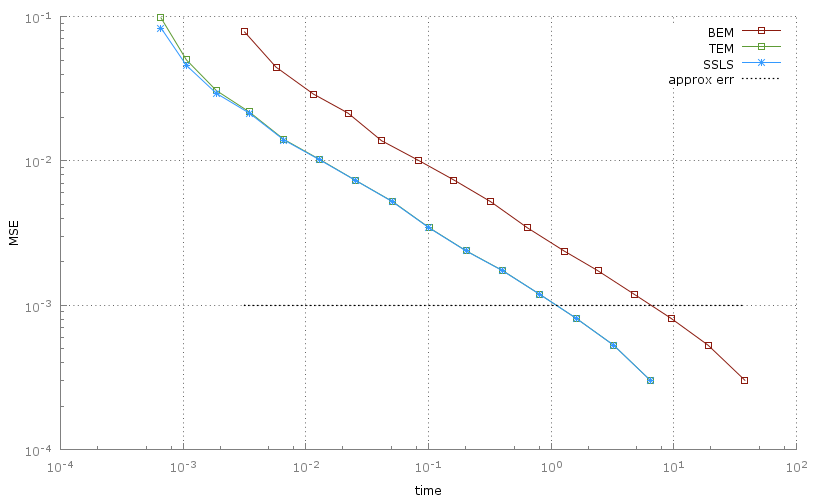
\includegraphics[width=0.7\linewidth]{./papers/paperB/figures/MSETime2}
		\caption{}
		\label{fig:MSETime2}
	\end{figure}
\subsection{Positivity of solutions}
First we consider the Lotka Volterra equation \cite{Mao2007a}
\begin{equation}\label{eqn:LotkaVolterra}
	dy(t)= \left[by(t)-a y(t)^2\right]dt + \sigma y(t) dW_t,
\end{equation}
which have exact solution
\begin{equation}\label{eqn:LotkaVolterraSol}
	y(t) = \frac{
		y_0
		\exp\left[
		b-\frac{1}{2}\sigma^2) t
		+\sigma W_t
		\right]
		}{
		\displaystyle
		1+a 
		y_0
		\int_0^t
		\exp\left[
		(b -\frac{1}{2})s
		+\sigma W_s
		\right]ds
	}.
\end{equation}
\begin{figure}
	\centering
	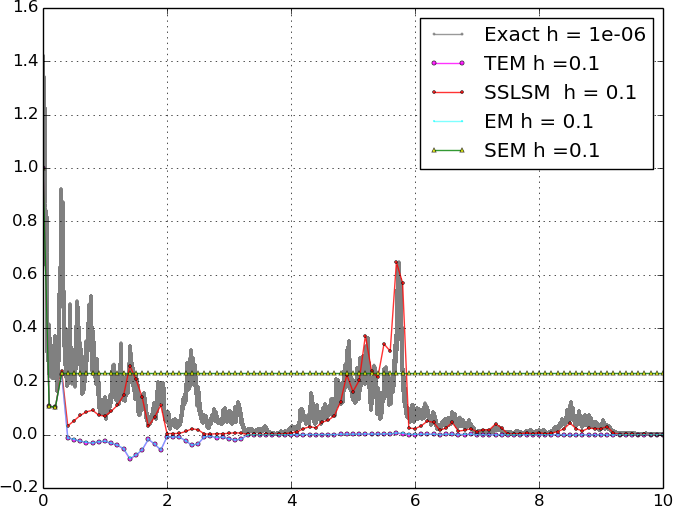
\includegraphics[width=0.7\linewidth]{./papers/paperB/figures/PathsLVEv4}
	\caption{}
	\label{fig:PathsLVEv4}
\end{figure}


	\appendix
	\begin{appendices}
		\section{Auxiliar results}
			In this appendix we enunciate basic results that are extensively used through our analysis. Here
the main reference are \cite{Shiryaev1996} and \cite{Mao2007}.
\begin{Holder}[{\cite[pg. 193]{Shiryaev1996}}]
	\begin{equation}\label{eqn:HolderInequality}
	\m[X^T Y] \leq
	\left(
	\m|X|^p
	\right)^{\frac{1}{p}}		
	\left(
	\m|X|^q
	\right)^{\frac{1}{q}}.
	\end{equation}
\end{Holder}

\begin{Young}[{\cite[pg. 111]{Hardy1934}}]
	\begin{equation}\label{eqn:YoungsInequality}
	|a||b| 
	\leq
	\frac{\delta}{p} |a|^p
	+\frac{\delta}{q \delta^{q/p}} |b|^q.
	\end{equation}
\end{Young}
%
\begin{Minkowski}[{\cite[pg. 194]{Shiryaev1996}}]
	\begin{equation}
	\left(
	\m |X+Y|^p
	\right)^{\frac{1}{p}}
	\leq
	\left(
	\m |X|^p
	\right)^{\frac{1}{p}}
	+
	\left(
	\m |Y|^p
	\right)^{\frac{1}{p}}.
	\end{equation}
\end{Minkowski}
%
%
\begin{Standard}
		Fix $1<p<\infty$ and consider a sequence of real numbers $\{a_i\}_{i=1}^{N}$  with $N \in \N$. Then one can 
	formulate this usefully inequality
	\begin{equation}\label{eqn:SingleHolder}
	\left(
	\sum_{j=1}^N a_j
	\right)^p
	\leq
	N^{p-1}
	\sum_{j=1}^{N}
	a_j^p.
	\end{equation}
\end{Standard}
%
\begin{Doobs}[{\cite[Thm. 3.5]{Mao2007}}]
%\begin{thm}[Doob's Martingale Inequality]
	Let $\{M_t\}_{t\geq 0}$ be a $\mathbb{R}^d$-valued martingale. Let $[a,b]$ be a bounded interval in $
	\mathbb{R}_{+}$.
	If $p>1$ and $M_t\in L^p(\Omega;\mathbb{R}^d)$ then
	\begin{equation}
	\label{eqn:DoobMartingaleInequality}
	\m\left( \sup_{a\leq t \leq b} |M_t|^p\right) 
	\leq \left(\frac{p}{p-1}\right)^p \m|M_b|^p. 
	\end{equation}
%\end{thm}
\end{Doobs}

\begin{bdg}[{\cite[Thm. 7.3]{Mao2007}}]
	Let $g\in \mathcal{L}(\mathbb{R}_+; \mathbb{R}^{d\times m})$. Define for $t\geq 0$
	\begin{equation}
		\label{thm:BDG}
		x(t) = \int_{0}^{t} g(s)dW(s) \quad \text{and } \qquad 
		A(t) = \int_{0}^{t} |g(s)|^2 ds.
	\end{equation}
	Then for all $p>0$, there exist universal positive constants $c_p$, $C_p$ such that
	\begin{equation}
		c_p\m|{A(t)}|^{\frac{p}{2}}
		\leq
		\m \left[
		\sup_{0\leq s \leq t} |x(s)|^p
		\right]
		\leq 
		C_p \m |A(t)|^{\frac{p}{2}},
	\end{equation}
	for all $t\geq 0$.  In particular, one may take
	\begin{align*}
	c_p &= (p/2)^p, & 			 C_p &= (32/p)^{\frac{p}{2}} & \text{if } 0<p<2; \\
	c_p &= 1,       & 			 C_p &= (32/p)^{\frac{p}{2}} & \text{if } p=2; \\
	c_p &= (2p)^{-\frac{p}{2}},& C_p &= \frac{p+1}{2(p-1)^{\frac{p}{2}}} & \text{if } p>2 .\\
	\end{align*}
\end{bdg}

\begin{Gronwall}[{\cite[Thm. 8.1]{Mao2007}}]
	Let $T > 0$ and $c \geq 0$. Let $u(\cdot)$ be a Borel measurable bounded nonnegative function on 
	$[0,T]$, and let $v$ be a nonnegative integrable function on $[0,T]$
	If
	$$
		u(t) \leq c 
		+\int_{0}^{t} v(s)u(s)ds \qquad \forall t \in [0,T],
	$$
	then
	\begin{equation}\label{thm:Gronwall}
		u(t) \leq c\exp
		\left(
		\int_{0}^{t} v(s)ds 
		\right)
		\qquad \forall t \in [0,T].
	\end{equation}
\end{Gronwall}
%
\begin{DiscreteGronwall}[{\cite[Lm. 3.4]{Mao2013}}]
	Let $M$ be a positive integer. Let $u_k$ and $v_k$ be non-negative numbers for $k=0,1,\dots,M$. 
	If
	$$
	u_k\leq u_0 + \sum_{j=0}^{k-1} u_j v_j
	$$
	then
	\begin{equation}
		\label{thm:DiscreteGronwall}
		u_k \leq u_0 
		\exp
		\left(
		\sum_{j=0}^{k-1}v_j
		\right).
	\end{equation}
\end{DiscreteGronwall}

	\end{appendices}
	\section*{\refname}
	\bibliographystyle{model2-names}
	\bibliography{library,Books}
\end{document}
